\RequirePackage[l2tabu, orthodox]{nag}
\documentclass{article}

\newcounter{chapter}
\setcounter{chapter}{2}

\setcounter{section}{\value{chapter}}
\addtocounter{section}{-1}

\usepackage{amssymb,amsmath,verbatim,graphicx,microtype,units,booktabs}
\usepackage[margin=10pt, font=small, labelfont=bf, labelsep=endash]{caption}
\usepackage[colorlinks=true, pdfborder={0 0 0}]{hyperref}
\usepackage[utf8]{inputenc}
\usepackage{pdfpages}

\usepackage[left=0.75in, right=0.75in]{geometry}
\usepackage{titleps}
\newpagestyle{main}{
    \setheadrule{.4pt}
    \sethead{Chapter \thechapter: \sectiontitle}
            {}
            {Illya Starikov}
}
\pagestyle{main}

\begin{document}
\section{Experiments}

\subsection{Study Guide Material}
\begin{description}
    \item [Hypothesis]
    \item [Steps in scientific investigation]
    \item [Independent variable] a variable (often denoted by x) whose variation does not depend on that of another.
    \item [Dependent variable] Affected by manipulating the independent variable.
    \item [Correlation]
    \item [Naturalistic observation] a researcher engages in careful observation of behavior without intervening directly with the subjects. Jane Goodall.
    \item [Reactivity] occurs when a subject’s behavior is altered by the presence of an observer.
    \item [Case study] An in-depth investigation of a particular subject.
    \item [Survey] researchers use questionnaires or interviews to gather information about specific aspects of participants’ background, attitudes, beliefs, or behavior.
    \item [Placebo effects]
    \item [Social desirability bias] a tendency to give socially approved answers to questions about oneself.
    \item [Experimenter bias]
    \item [6 APA ethical guidelines] The ethics issues that we have discussed in this section have led the APA to develop a set of ethical standards for researchers (American Psychological Association, 2002). Some of the most important guidelines for research with human participants include the following:
    \begin{enumerate}
        \item  people's participation in research should always be voluntary and they should be allowed to withdraw from a study at any time
        \item  participants should not be subjected to harmful or dangerous treatments
        \item if a study requires deception, participants should be debriefed (informed of the true nature and purpose of the research) as soon as possible
        \item and participants’ right to privacy should never be compromised.
    \end{enumerate}

    Guidelines for research with animals include:
    \begin{enumerate}
        \item harmful or painful procedures cannot be justified unless the potential benefits of the research are substantial;
        \item research animals are entitled to decent living conditions.
    \end{enumerate}
\end{description}

\subsection{Book Notes}
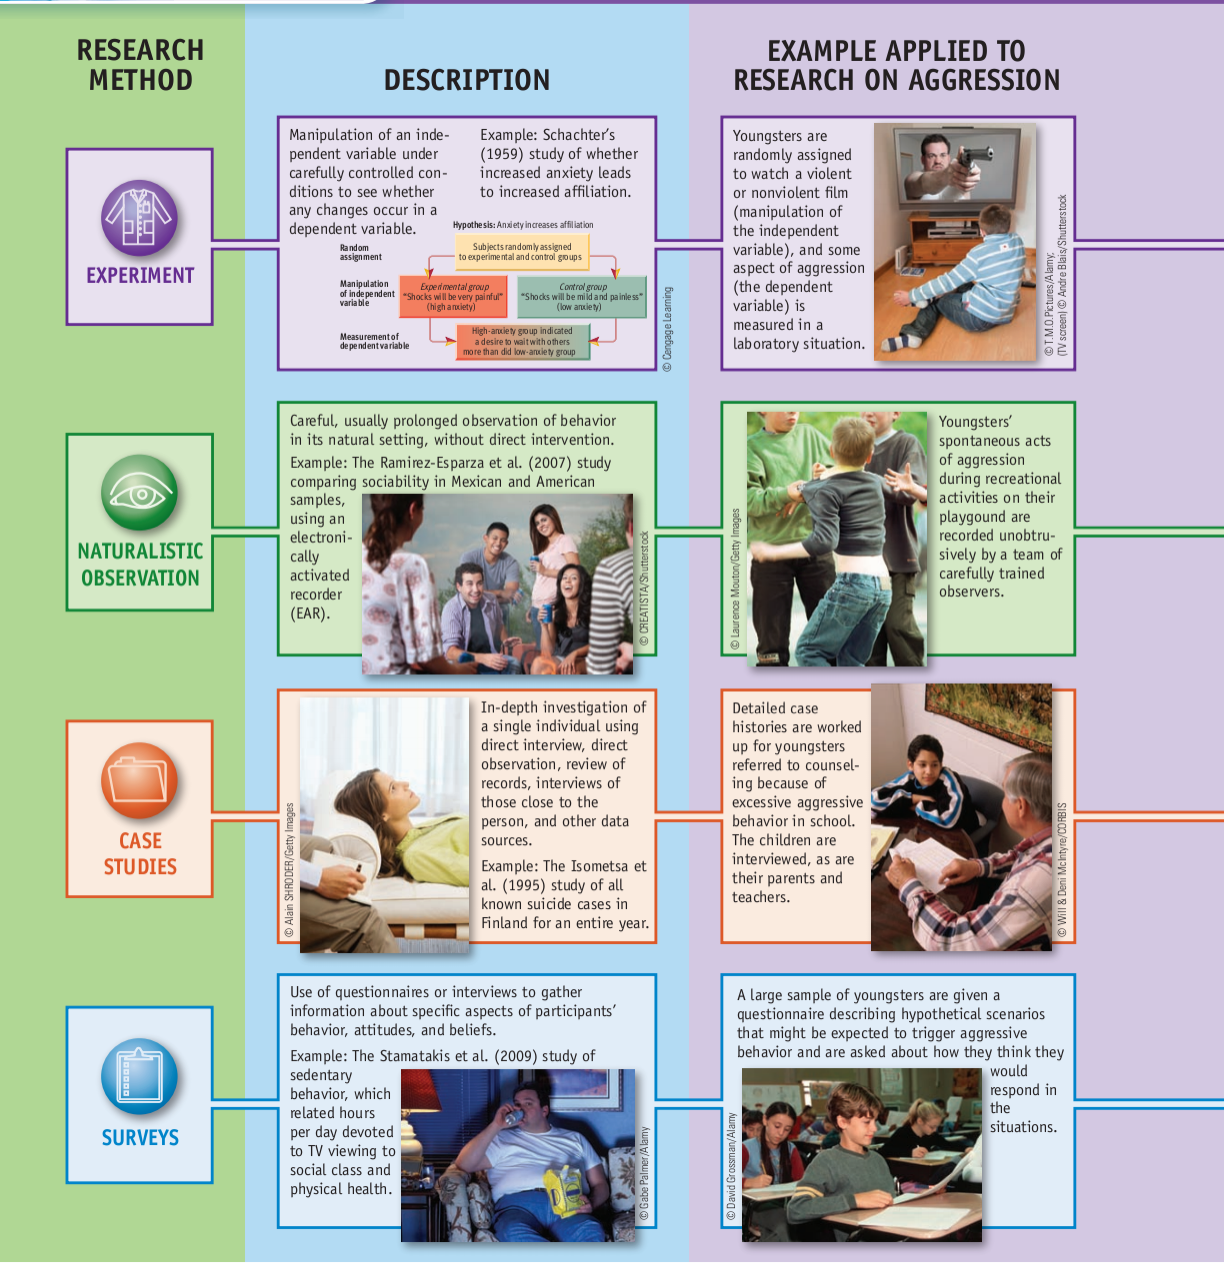
\includegraphics[width=\textwidth]{methods}
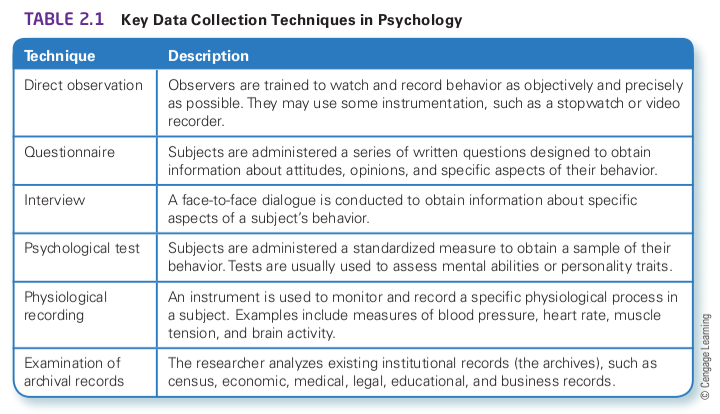
\includegraphics[width=\textwidth]{data_collection}

\subsection{Powerpoint Notes}
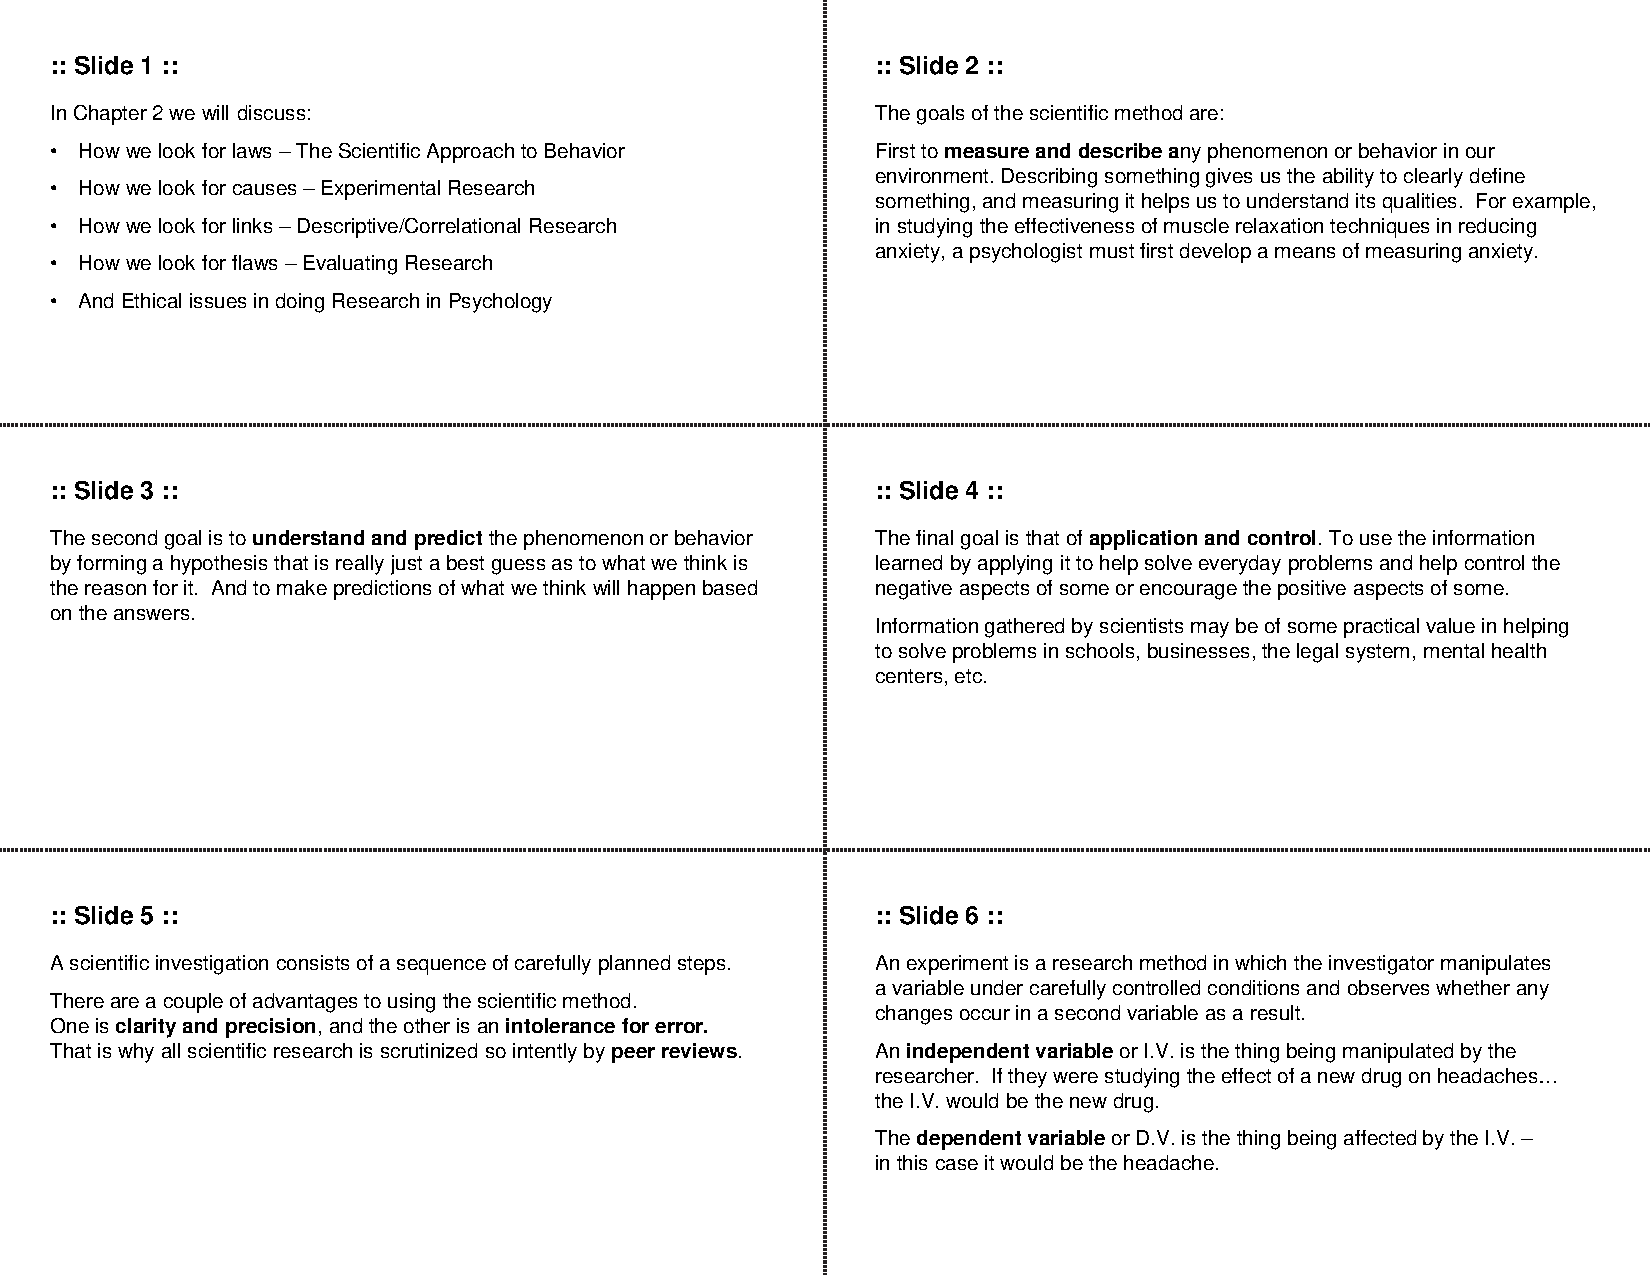
\includepdf[width=1.15\textwidth, pages=-]{lecture_notes.pdf}

\end{document}